\documentclass[../main.tex]{subfiles}
\begin{document}
\chapter{Lecture 6 - 07-04-2020}

$(X, Y)$ We random variables drawn iid from $D$ on $X \cdot Y$ $\longrightarrow$ where $D$ is fixed but unknown\\\\
Independence does not hold. We do not collect datapoints to an independent
process.\\
Example: identify new article and i want to put categories. The feed is highly
depend on what is happening in the world and there are some news highly
correlated. Why do we make an assumption that follows reality?
Is very convenient in mathematical term.
If you assume Independence you can make a lot of process in mathematical
term in making the algorithm.\\
If you have enough data they look independent enough. Statistical learning is
not the only way of analyse algorithms —> we will see in linear ML algorithm
and at the end you can use both statistical model s

\section{Bayes Optimal Predictor}

$$ f^* : X \rightarrow Y$$
$$ f^*(x) = argmin \, \barra{E}\left[ \, \ell(y,\hat{y})| X=x \, \right] \qquad \hat{y} \in Y$$
\\
In general $Y$ given $X$ has distribution $D_y|X=x$
\\
Clearly $\forall$ $h$ \quad $X\rightarrow Y$
\\
$$
\barra{E} \left[ \, \ell(y, f^*(x)) | X=x \, \right] \leq \barra{E}\left[ \, \ell(y,h(x)| X = x \, \right] 
$$
$$
X,Y \qquad \barra{E} \left[ \, Y|X = x \, \right] = F(x) \quad \longrightarrow \red{Conditional Expectation} 
$$
$$
\barra{E} \left[ \, \barra{E} \left[ \, Y|X \, \right] \, \right] = \barra{E}(Y)
$$
\\
Now take Expectation for distribution
$$
\barra{E} \left[ \, \ell(y, f^*(x))\, \right] \leq \left[ \, \barra{E} (\ell(y, h(x)) \, \right]
$$
\\ where \red{risk is smaller in $f^*$}
\\
I can look at the quantity before\\
$l_d$ Bayes risk $\longrightarrow$ Smallest possible risk given a learning problm
\\\\
$$
l_d(f^*) > 0 \qquad \textit{because y are still stochastic given X}
$$
\\
Learning problem can be complem $\rightarrow$ large risk
\\\\
\subsection{Square Loss}
$$\ell(y,\hat{y} = (y - \hat{y})^2$$
I want to compute bayes optimal predictor\\
$\hat{y}, y \in \barra{R}$
\\
$$
f^*(x) = argmin \, \barra{E} \left[ \, (y-\hat{y})^2 | X = x \, \right] = \qquad \hat{y} \in \barra{R}
$$\
$$
\textit{we use }\qquad \barra{E}\left[\,X+Y\,\right] = \barra{E}[X] + \barra{E}[Y] = argmin \, \barra{E}\left[\,\red{y^2} + \hat{y}^2- 2\cdot y \cdot \hat{y}^2 | X = x \, \right] = 
$$
\\
Dropping $\red{y^2}$ i remove something that is not important for $\hat{y}$
\\
$$
= argmin ( \barra{E} \left[\, y^2 | X = x\, \right] + \hat{y}^2 - 2 \cdot \hat{y} \cdot \barra{E} \left[ \, y | X = x \, \right] ) = 
$$
$$
= argmin (\hat{y}^2 - 2 \cdot \hat{y} \cdot \barra{E} \left[ \, y | X = x \, \right] ) =
$$
\\ Expectation is a number, so it's a \red{constant}
\\
Assume $ \boxdot = y^2 $
$$
argmin \, \left[\, \boxdot + \hat{y}^2 + 2 \cdot \hat{y} \cdot \barra{E} \left[\, Y|X =x\,\right] \right]
$$
where red{$G(\hat{y})$ is equal to the part between $\left[...\right]$}
$$
\frac{d G(\hat{y})}{d\hat{y}} = 2 \cdot \hat{y}- 2 \cdot \barra{E} \left[ \, y | X= x \, \right] = 0  \quad \longrightarrow \quad \red{\textit{So setting derivative to 0}}
$$
\\ --- DISEGNO OPT CURVE ---\\\\
$G' (\hat{y}) = \hat{y}^2 - 2\cdot b \cdot \hat{y}$
\\
$$
\hat{y} = \barra{E} \left[ \, y| X= x \, \right] \qquad f^*(x) = \barra{E} \left[ \, y | X = x \, \right]
$$
\\
Square loss is nice because expected prediction is ...\\
In order to predict the best possibile we have to estimate the value given data
point.
\\
$$ 
\barra{E} \left[ \, (y- f^*(x))^2 | X = x \, \right] = 
$$
$$
= \barra{E} \left[ \, (y- \barra{E} \left[ \, y | X = x \,\right] )^2 | X = x \, \right] = Var \left[ \, Y | X = x \, \right]
$$
\\
\subsection{Zero-one loss for binary classification}
$ Y = \{-1,1\}
$
$$
\ell(y,\hat{y}) = I \{ \hat{y} \neq y \} 
\qquad I_A (x) = 
\begin{cases}
1 \quad  x \in A
\\
0 \quad  x \not\in A
\end{cases}
$$
\\
\red{If $\hat{y} \neq y$ true, indicator function will give us 1, otherwise it will give 0}
\\
$$
D \quad on \qquad X \cdot Y \qquad D_x^* \quad D_{y|x} = D
$$\
$$
D_x \qquad \eta: X \longrightarrow \left[ \, 0,1 \, \right] \qquad \eta = \barra{P} \,(y = 1 | X = x )
$$\
$$
D \leadsto (D_x, \eta) \quad \longrightarrow \quad \red{\textit{Distribution 0-1 loss}}
$$\
$$
X \backsim D_x \quad \longrightarrow \quad \red{ \textit{Where $\backsim$ mean "draw from" and $D_x$ is marginal distribution} }  
$$
$$
Y = 1 \qquad \textit{   with probability } \eta(x)
$$\
$$
D_{y|x} = \{ \eta(x), 1- \eta(x) \}
$$
\\
Suppose we have a learning domain\\
--- DISEGNO --
\\
where $\eta$ is a function of $x$, so i can plot it\\
$\eta$ will te me $Prob (x) = $
\\
$\eta$ tells me a lot how hard is learning problem in the domain
\\
$\eta(x)$ is not necessary continous
\\
--- DISEGNO ---
\\\\
$\eta(x) \in \{0,1\} $ \qquad $y$ is always determined by $x$
\\
How to get $f^*$ from the graph?
\\
$$
f^+ : X \rightarrow \{-1,1\}
$$
$$
Y = \{-1, +1 \}
$$
--- DISEGNO ---\\
===============================\\
MANCA ROBAAAAAAAAAAAAAAAAAAAAAAAAAAAAA\\
==============================
$$
f^*(x) = argmin \, \barra{E} \left[ \,  \ell(y, \hat{y}) | X= x\, \right] =  \qquad \longrightarrow \hat{y} \in \{-1,+1 \}
$$
$$
= argmin \,  \barra{E} \left[ \, I\{\hat{y} = 1\} \cdot I\{Y=-1\} + I\{\hat{y}=-1\} \cdot I\{y=1\} \, | \, X = x \, \right] =
$$
\\
we are splitting wrong cases
\\
$$
= argmin \, (  \, I\{\hat{y} = 1\} \cdot \barra{E} \left[ \, I\{Y=-1\} |\, X = x\, \right] + I\{\hat{y}=-1\} \cdot \barra{E} \left[ \, I\{y=1\} \, | \, X = x \, \right] \, ) =  \quad \red{\divideontimes}
$$\\
We know that: $$ \barra{E} \left[ \, I \{y = -1 \} \, | \, X = x \, \right] = 1 \cdot \barra{P} \\ (\hat{y} = -1 | X = x ) + 0 \cdot \barra{P} (y = 1 | X= x) =  
$$
$$
\barra{P} (x = -1 | X=x ) = \, \red{ 1- \eta(x) }
$$\\
$$
 \red{\divideontimes} =   argmin \, (  \, \col{I\{\hat{y} = 1\} \cdot (1 - \eta(x))}{Blue} + \col{I \{ \hat{y} = -1\} \cdot (\eta(x)}{Orange} \, )
$$
where \col{Blue}{Blue} colored $I \{...\} = 1$° and \col{Orange}{Orange} $I \{...\} = 2$°
\\\\
I have to choose \red{-1 or +1 } so we will \textbf{remove one of the two (1° or 2°) }
\\
It depend on $\eta(x)$:
\begin{itemize}
\item  If $\eta(x) < \frac{1}{2}$ \quad $\longrightarrow$ \quad kill 1°
\item  Else $\eta(x) \geq \frac{1}{2}$ \quad $\longrightarrow$ \quad kill 2°
\end{itemize}
$$
f^*(x) = 
\begin{cases}
+1 \qquad if \, \eta(x) \geq \frac{1}{2}\\
-1 \qquad if \, \eta(x) < \frac{1}{2}
\end{cases}
$$
\section{Bayes Risk}

$$
\barra{E} \left[ \, I \{ y \neq f^*(x) \}\, | \, X = x \, \right] = \barra{P}(y \neq f^*(x)|X= x)
$$\
$$
\eta(x) \geq \frac{1}{2} \quad \Rightarrow \quad \hat{y} = 1  \quad \Rightarrow \quad  \barra{P} (y \neq 1 | X= x) = 1-\eta(x)
$$\
$$
\eta(x) < \frac{1}{2} \quad \Rightarrow \quad \hat{y} = -1  \quad \Rightarrow \quad  \barra{P} (y \neq 1 | X= x) = \eta(x) \quad
$$
\\
Conditiona risk for 0-1 loss is:
\\
$$
\barra{E} \left[ \, \ell (y, f^*(x)) \, | \, X = x \, \right] 
\quad = \quad I \{ \eta(x) \geq \frac{1}{2}\} \cdot(1-\eta(x)) + I \{ \eta(x) <\frac{1}{2}\} \cdot \eta(x) = 
$$
$$
 = min \, \{ \eta(x), 1- \eta(x) \}
$$\
$$
\barra{E} \left[ \, \ell , f^*(x) \, \right] = \barra{E} \left[ \, min \, \{ \eta(x) , 1- \eta(x) \} \, \right] 
$$
\begin{figure}[h]
    \centering
    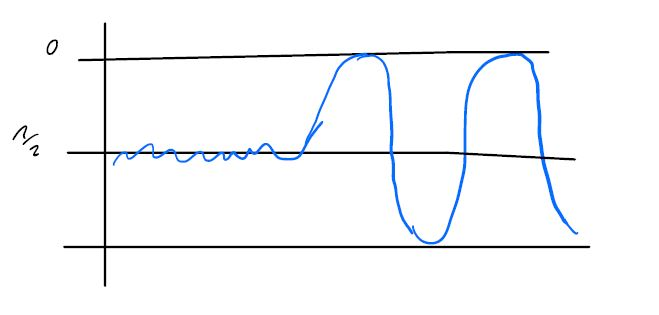
\includegraphics[width=1\textwidth]{bayesrisk.jpg}
    \caption{Example of Bayes Risk}
    %\label{fig:}
\end{figure}
\\
Conditional risk will be high aroun the half so min between the two is around
the half since the labels are random i will get an error near $50\%$.\\
My condition risk will be 0 in the region in the bottom since label are going to
be deterministic.
\end{document}
